\documentclass[a4paper,10pt]{report}
\usepackage[utf8]{inputenc}  
\usepackage[T1]{fontenc}
\usepackage{graphicx}
\usepackage{tikz}
\usepackage[top=3cm, bottom=3cm, left=3cm, right=3cm]{geometry}
\usepackage{hyperref}

\DeclareUnicodeCharacter{00A0}{ }
\widowpenalty=10000
\clubpenalty=10000
\input{environnements.tex}
\setlength{\parindent}{0.5cm}
\begin{document}

\title{Projet Imagerie Multispectrale}
\author{Aurélien Barbotin Pierre David Benjamin Michelland Youna le Vaou}

\maketitle

\chapter{Présentation du projet}
\documentclass[a4paper,10pt]{article}
\usepackage[utf8x]{inputenc}
\usepackage{url}
\usepackage{graphicx}
\usepackage{array}

%opening
\title{Etat de lard}
\author{Aurélien Barbotin Pierre David Benjamin Michelland Youna le Vaou}

\begin{document}

\maketitle

\section{État de l'art}
\subsection{Imagerie satellite hyperspectrale}

Jusqu'à récemment, la principale source d'images satellite hyperspectrales exploitées par les scientifiques étaient les satellites MODIS (Moderate-Resolution Imaging SpectroRadiometer). Ces deux satellites, lancés par la NASA en 1999 et 2002, imagent l'intégralité de la surface de la terre tous les deux jours. Ces satellites sont capables de mesurer 36 bandes fréquentielles avec trois résolutions différentes : 250m, 500m et 1000m\cite{nasa}. L'objectif de cette mission est de ``jouer un rôle vital dans le développement de modèles globaux, validés et interactifs de systèmes terrestres capables de prévoir des changements globaux avec suffisamment de précision pour aider les décideurs politiques à prendre des décisions avisées concernant la protection de notre environnement.''

Ces données ont ainsi pu servir à analyser la qualité de l'air au niveau du sol et, entre autres, d'en déduire la présence d'évènements exceptionnels comme des feux de forêt ou du brouillard\cite{airSurv}. A l'aide d'indices comme le NDVI (normalized difference vegetation index) calculés à partir de données hyperspectrales, il est possible d'établir la présence ou l'absence de végétation dans une zone. En effet, les plantes chlorophyliennes absorbent fortement la lumière rouge et réfléchissent la lumière proche infrarouge : la différence normalisée d'intensité entre ces deux bandes correspond à l'indice NDVI dont une valeur proche de 1 indique la présence de végétation, et une valeur proche de 0 son absence. De multiples applications, comme l'étude de la désertification de zones dues à l'activité humaine\cite{desert} ont dores et déjà été mises en évidence.

La faible résolution des données MODIS ne permet en revanche pas de discerner des détails comme des cours d'eau ou des habitations, et des données plus précises sont donc nécessaires pour obtenir de meilleures classifications. 

Dans le cadre du projet \textit{Copernicus} d'observation de la Terre, l'agence spatiale européenne (ESA) développe en ce moment les missions Sentinel. Chacune de ces missions consiste en une paire de satellite en orbite autour de notre planète, récoltant des données sur la surface et l'atmosphère. Ainsi, les satellites Sentinel 2 (Sentinel 2-A lancé le 23 juin 2015 et 2-B dont le lancement est prévu pour la seconde moitié de 2016)\cite{sent2} récoltent des données hyperspectrales sur 13 bandes de fréquence : 4 bandes avec une résolution de 10m et 9 avec une résolution de 60m.

Les données Sentinel 2 étant très récentes, nous faisons partie des premiers à les analyser et aucun article à leur sujet n'a encore été publié à notre connaissance. Leur analyse et leur classification relève donc de la recherche.

\section{Résultats}
Dans un but de répétabilité, nous avons testé et optimisé toutes nos méthodes de machine learning sur une unique image hyperspectrale (dont une vue en RGB est donnée en figure \ref{fig:veniseRGB}).
\begin{figure}
  \centering
    \includegraphics[width=0.5\textwidth]{venise}
  \caption{Image hyperspectralde de Venise qui nous a servi de référence (vue en RGB)}
  \label{fig:veniseRGB}
\end{figure}
Le résultat d'une classification est une image RGB dont la couleur de chaque pixel représente la classe à laquelle il appartient selon l'algorithme. Par exemple, dans une image résultat, un pixel bleu correspond à un point indentifé par l'algorithme comme étant de l'eau. Notre code couleur est résumé dans le tableau \ref{table:codeCouleur}.
\begin{figure}
 \begin{center}
  \begin{tabular}{|c|c|}
    \hline
    Nature du terrain & couleur \\
    \hline
  Champ & Vert \\
  Ville &  Rouge \\
  Eau &  Bleu \\
  Boue & Marron \\
    \hline
  \label{table:codeCouleur}
  \end{tabular}
\caption{Code couleur des images produites par machine learning.} 
\end{center}
\end{figure}
Estimer la qualité d'un classificateur revient à estimer la qualité de l'image résultante. Pour cela, deux méthodes s'offrent à nous: la première numérique, consiste à calculer la matrice de confusion de chaque classificateur comme expliqué INSERER ICI OU CEST EXPLIQUE. L'autre méthode consiste à estimer à l'oeil la correspondance entre les prédictions de nos algorithmes et la réalité (les zones de référence étant elles-mêmes choisies à l'oeil, ce critère n'est pas plus mauvais que l'autre). Pour immédiatement visualiser cette correspondance, nous superposons l'image de base avec l'image résultante en transparence, comme par exemple sur la figure \ref{fig:veniseLSE}.

\subsection{classificateur linéaire}
\label{lineaire}
La première classification que nous testée est aussi la seule que nous avons entièrement implémentée nous mêmes. Il s'agit de classification à l'aide d'un classificateur linéaire. Les résultats obtenus sont encourageants, avec une première classification qui à première vue correspond à la répartition réelle des trois classes étudiées (figure \ref{fig:veniseLSE} avec la matrice de confusion correspondante \ref{table:confknn}).

\begin{figure}
  \centering
    \includegraphics[width=0.5\textwidth]{veniseLSE}
  \caption{Résutat de classification avec un classificateur linéaire}
  \label{fig:veniseLSE}
\end{figure}

\begin{figure}
\begin{center}
 \begin{tabular}{|c|c|c|c|c|}
  \hline
  Nature du terrain & Ville & Champ & Eau & Rappel \\
  \hline
Ville & 5309   &   878    &   15 & 0.856014 \\
Champ & 1296   &  9832     &   0  & 0.883537 \\
Eau &  2   &     0  &   6350 & 0.999685 \\
Précision & 0.803542  & 0.918021 & 0.997643 & 0.907483 \\
  \hline
\end{tabular}
\end{center}
\caption{Matrice de confusion de la classification linéaire}
\label{table:confknn}
\end{figure}

La précision totale de cette méthode est de 90.7\%. On peut constater que l'eau est très bien classifiée, et que les erreurs proviennent majoritairement de confusions entre les champs et la ville.

\subsection{LDA: Analyse linéaire de discriminant}
La classification LDA, pour Linear Discriminant Analysis (Analyse linéaire de discriminant) suppose une distribution gaussienne des points au sein de chacune des classes. Or, nous avons choisi des polygones de manière à ce qu'ils contiennent le moins de points possibles, le plus représentatifs possibles, afin de diminuer les temps de calcul. Ce faisant, on n'a pas pris un échantillon continu de points et l'approximation gaussienne est difficilement valable, ce qui explique les mauvais résultats obtenus, en particulier sur les zones de ville.
\begin{figure}
  \centering
    \includegraphics[width=0.5\textwidth]{venise+LDA}
  \caption{Résutat de classification avec une analyse linéaire de discriminant}
  \label{fig:veniseLDA}
\end{figure}

\begin{table}
\begin{center}
 \begin{tabular}{|c|c|c|c|c|}
  \hline
  Nature du terrain & Ville & Champ & Eau & Rappel \\
  \hline
Ville & 2026  &   4176  &      0 & 0.326669 \\
Champ & 675  &  10453   &     0 & 0.9393427 \\
Eau &  0    &    0  &   6352   &     1 \\
Précision & 0.750093 & 0.71454  &      1 & 0.795161\\
  \hline
\end{tabular}
\end{center}
\caption{Matrice de confusion de l'analyse avec discriminant linéaire }
\label{table:veniseLDA}
\end{table}
    
     

\subsection{méthode knn:k-nearest-neighbours ou k plus proches voisins}
La méthode des k-nearest neighbors présente des résultats intéressants, et nous avons obtenu une classification très précise avec cette méthode. Nous avons testé cette méthode avec différentes valeurs de k (1, 3, 20, 200) et il s'est avéré que cette valeur n'influait pas sur la classification, ce qui nous laisse penser que les points sont naturellement bien séparés. Nous avons donc choisi de faire notre classification avec la valeur du paramètre k=1. Les résultats obtenus sont montrés sur la figure \ref{fig:1NN} et le tableau \ref{table:1NN}.
\begin{table}
\begin{center}
 \begin{tabular}{|c|c|c|c|c|}
  \hline
  Nature du terrain & champ & ville & eau & Rappel \\
  \hline
Champ & 9929 & 71 & 	0 &	99.29 \\
Ville & 540 &	9460 &	0 &	94.6 \\
Eau &  0 &	0 &	10000 &	100 \\
Précision & 99.29 & 94.6 & 100 & 97.96 \\
  \hline
\end{tabular}
\end{center}
\label{table:1NN}
\caption{Matrice de confusion de l'algorithme de 1-plus proche voisin.}
\end{table}

\begin{figure}
  \centering
    \includegraphics[width=0.5\textwidth]{resultat1NN}
  \caption{Résutat de classification avec la méthode du 1-plus proche voisin}
  \label{fig:1NN}
\end{figure}

\subsection{Support Vecteur Machine}
Cette méthode utilise deux métaparamètres : C et $\gamma$. Afin d'optimiser l'apprentissage et la classification de notre image, il faut donc trouver les métaparamètres idéaux. Pour cela, on fait un ensemble de validations croisées dans lequel on sépare notre jeu de données en 5, 4 parts servant à l'apprentissage et la dernière part au test. On fait ce test 100 fois pour 100 couples de valeurs (C,$\gamma$), et le jeu de paramètres obtenant le meilleur score de précision lors de la validation croisée correspondaux paramètres que l'on utilisera. Afin de déterminer d'un seul coup d'oeil si l'on a trouvé un set de paramètres optimal, on représente les résultats des différentes validations croisées sur une courbe en deux dimensions (figure \ref{fig:crossMap}).

\begin{figure}
  \centering
    \includegraphics[width=0.5\textwidth]{crossValLog}
  \caption{Scores obtenus pouf 100 validations croisées avec différents couples de paramètres (C,$\gamma$). La couleur d'un point correspond à la précision moyenne de l'algorithme pour le couple (C,$\gamma$) qui lui sert de coordonnées. Les axes sont en échelle logarithmique.}
  \label{fig:crossMap}
\end{figure}

Cette figure qu'en effet, la précision de l'algorithme dépend du choix judicieux des métaparamètres. Le meilleur choix de métaparamètres dans notre cas est le couple (C,$\gamma$)=(1,$ 10^{-3}$). Nous obtenons alors l'image \ref{fig:veniseSVM}et la matrice de confusion \ref{table:SVC}.

\begin{table}
\begin{center}
 \begin{tabular}{|c|c|c|c|c|}
  \hline
  Nature du terrain & Ville & Champ & eau & Rappel \\
  \hline
Ville & 9867 & 133 & 	0 &	98.67 \\
Champ & 159 &	9841 &	0 &	98.41 \\
Eau &  38 &	0 &	9962 &	99,62 \\
Précision & 98.04 & 98.6 & 100 & 98.9 \\
  \hline
  \end{tabular}
\end{center}
\label{table:SVC}
\caption{Matrice de confusion de l'algorithme de Support Vecteur Machine.}
\end{table}

\begin{figure}
  \centering
    \includegraphics[width=0.5\textwidth]{veniseSVM}
  \caption{Résutat de classification avec le support vecteur machine.}
  \label{fig:veniseSVM}
\end{figure}

\subsection{Conclusion}
La première conclusion que nous pouvons tirer de notre travail est que les méthodes de machine learning que nous avons testées donnent pour la plupart des résultats très satisfaisants. Le support vecteur machine en particulier nous fournit une accuracy de 98.9\% avec trois classes. Il est d'usage de prétraiter les données pour calculer des indices comme l'index de végétation différentiel normalisé (NDVI)\cite{NDVI}:
\begin{equation}
NDVI=\frac{NIR-VIS}{NIR+VIS}
\end{equation}
Où NIR correspond à l'intensité lumineuse dans le proche infrarouge et VIS dans le rouge. Une valeur de cet indice proche de 1 indique la présence de végétation, une valeur négative indique des nages ou l'absence de végétation. Dans notre cas, les images multispectrales fournissent suffisamment d'informations par elles-mêmes pour classifier les sols avec précision sans passer par cet indice.

Nous avons également démontré que chacune des 12 bandes est nécessaire dans la classification, puisque la perte de l'une d'entre elles entraîne une baisse significative de l'accuracy comme on l'a vu dans le paragraphe \ref{lineaire}.

\subsection{Limites et améliorations}
Nous avons constaté que la boue le long des côtes n'est pas toujours reconnue de la même manière par nos algorithmes: parfois champs, parfois ville, ils ne correspondent à aucune de nos trois classes. Il est en effet rare en apprentissage automatique d'utiliser seulement trois classes. Nous avons donc rajouté une classe ``boue'' et testé certaines de nos classifications dessus, en particulier le Support Vecteur Machine. Le résultat est donné en figure \ref{fig:SVM4Cl}. La boue est bien classifiée mais l'introduction de cette 4e classe entraîne l'apparition de faux positifs, en particulier dans les champs dont la réponse spectrale est proche.
\begin{figure}
  \centering
    \includegraphics[width=0.5\textwidth]{SVM4Classes}
  \caption{Résutat de classification de 4 classes avec le support vecteur machine.}
  \label{fig:SVM4Cl}
\end{figure}

Plusieurs méthodes s'offrent à nous pour améliorer ce résultat de classification: la plus simple, appelée \textit{whitening} (blanchissement, en français) consiste à centrer chaque bande spectrale sur sa moyenne et à la dilater proportionnellement à son écart-type. Cette méthode renormalise les distributions et permet une meilleure classification.

Il est également possible d'ajouter encore plus d'informations, en utilisant les données de satellites Sentinel-1 qui sont des images radar. Une dernière méthode tout juste mise au point par notre tuteur N. Brodu consiste à améliorer la résolution des bandes spectrales de plus faible résolution en 

Enfin, les données sentinel-2 étant toutes nouvelles, peu de scènes sont à notre disposition. Nous n'avons donc que très peu testé nos algorithmes de classification sur des zones différentes de notre zone test. Il serait intéressant de vérifier que la classification fonctionne sur d'autres zones sans avoir besoin de redéfinir des polygones d'apprentissage.

\bibliography{Biblio}
\bibliographystyle{plain}
\end{document}

\section{Machine Learning}
\textit{L'apprentissage automatique (machine learning en anglais), champ d'étude de l'intelligence artificielle, concerne la conception, l'analyse, le développement et l'implémentation de méthodes permettant à une machine (au sens large) d'évoluer par un processus systématique, et ainsi de remplir des tâches difficiles ou impossibles à remplir par des moyens algorithmiques plus classiques.\footnote{\href{https://fr.wikipedia.org/wiki/Apprentissage_automatique}{Apprentissage automatique}}}
\paragraph{}
Le machine learning se sépare en trois type d'apprentissage :
\begin{itemize}
  \item[>] L'apprentissage non-supervisés, qui consiste à donner à notre algorithme uniquement les données à classifier et à le laisser établir les différentes classes à partir des ensembles qui se séparent le mieux.
  \item[>] Les régressions qui cherchent à définir les données à l'aide d'une loi mathématique.
  \item[>] Les apprentissages supervisés, pour lesquels il faut définir en plus des données à traiter, des ensembles de vecteurs représentatifs de chacune des classes et déjà classé. Les vecteurs classés manuellement vont servir d’entraînement pour l'apprentissage et donc pour trouver les frontières qui séparent le mieux nos différentes classes.
\end{itemize}
\subsection{Les principes}
\paragraph{}
Dans Le cas de la surveillance d'occupation des sols, on utilise souvent des méthodes supervisées, car il est relativement aisé de reconnaître à l'œil les différents types de zones au sol (eau, champs, villes, ...). Là encore, il existe plusieurs familles d'algorithmes d'apprentissage supervisé, on différenciera dans un premier temps les algorithmes linéaires et non-linéaires. Dans la famille des algorithmes non-linéaire, on trouve des algorithmes intrinsèquement multi-classes (tel que l'algorithme dit des k-plus proches voisins que nous détaillerons plus tard), et les algorithmes binaires.
\begin{center}
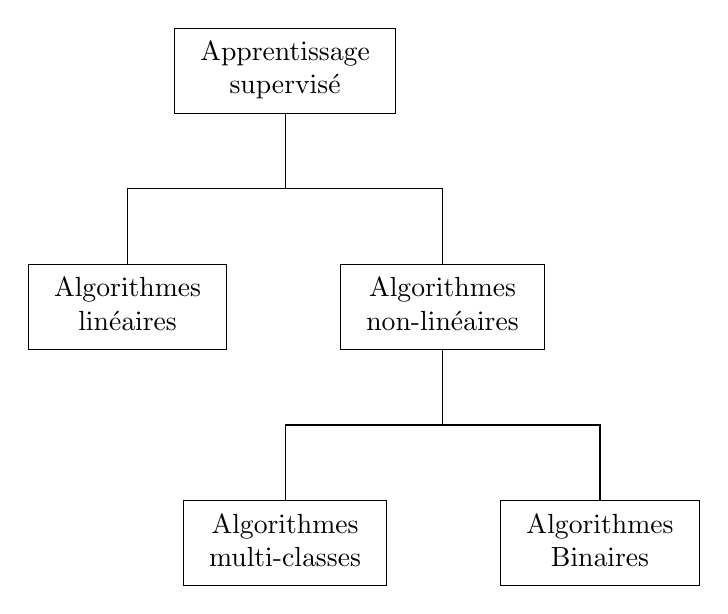
\begin{tikzpicture}
\begin{scope}
\node (AS) at (0,6) [rectangle,draw] {\begin{tabular}{c}Apprentissage\\ supervisé\end{tabular} };
\node (ASL) at (-2,3) [rectangle,draw] {\begin{tabular}{c}Algorithmes\\ linéaires\end{tabular} };
\node (ASNL) at (2,3) [rectangle,draw] {\begin{tabular}{c}Algorithmes\\ non-linéaires\end{tabular} };
\node (ASIM) at (0,0) [rectangle,draw] {\begin{tabular}{c}Algorithmes\\ multi-classes\end{tabular} };
\node (ASNM) at (4,0) [rectangle,draw] {\begin{tabular}{c}Algorithmes\\Binaires\end{tabular} };
\draw (AS) -- (0,4.5);
\draw (0,4.5) -| (ASNL);
\draw (0,4.5) -| (ASL);
\draw (ASNL) -- (2,1.5);
\draw (2,1.5) -| (ASIM);
\draw (2,1.5) -| (ASNM);
\end{scope}
\end{tikzpicture}
\end{center}
%pas sûr que le diagramme soit utile finalement...
\paragraph{}
Pour les algorithmes intrinsèquement multi-classes, il suffit de stocker les vecteurs d’entraînement et d'appliquer directement la classification à l'ensemble des données, il n'y a donc pas d’entraînement à proprement parler.
\paragraph{}
Les algorithmes binaires, quant à eux demandent un peu plus de travail, dès que l'on veut traiter plus de deux classes, il faut faire plusieurs entraînements, en se ramenant chaque fois à un problème binaire. Là encore, il y a deux approches possibles en fonction des algorithmes :
 \begin{itemize}
   \item[>] La première approche s'appelle "un contre tous", elle consiste comme son nom l'indique, à prendre chaque classe et à l'opposer à l'ensemble des autres classes. On obtient alors n problèmes binaires et pour un élément à classifier, en cas d'ambiguïté, la classe qui obtient le plus de "votes" favorables est choisie;
   \item[>] La seconde méthode est le "un contre un", toutes les classes sont "opposées" successivement, deux à deux, et de la même façon c'est la classe qui obtient le plus de "votes" favorables qui est choisie. La principale différence réside dans le fait qu'il y ait dans ce cas ${n \choose 2}=\frac{n(n-1)}{2}$ entraînements à réaliser.
 \end{itemize}
 \subsection{Les algorithmes}
\paragraph{Les classifications linéaires\\}
Réaliser une classification linéaire d'un ensemble de données en différentes classes revient, en deux dimensions, à trouver la droite qui sépare au mieux deux ensembles de vecteurs.
\label{ClassLin}
\begin{center}
 \begin{tikzpicture}
 \begin{scope}
 \draw[latex-latex, thin, draw=gray] (-4,0)--(4,0) node [right] {$x$}; % l'axe des abscisses
 \draw[latex-latex, thin, draw=gray] (0,-4)--(0,4) node [above] {$y$}; % l'axe des ordonnées
 \draw[thick] (-4,-4)--(4,4); % la courbe

\foreach \Point in {(-2,2), (-2,1.8), (-2,2.2), (-1.5,2), (-1.8,2.2),(-1.5,2.2),(-1.8,2),(-2.2,2),(-2,1.5),(-1.8,1.8)}{
    \node [blue] at \Point {\textbullet};
}

\foreach \Point in {(2,-2), (2,-1.8), (2,-2.2), (1.5,-2), (1.8,-2.2),(1.5,-2.2),(1.8,-2),(2.2,-2),(2,-1.5),(1.8,-1.8)}{
    \node [red] at \Point {\textbullet};
}

% to ensure that the points are being properly centered:
\draw [dotted, gray] (-4,-4) grid (4,4);
 \end{scope}
\end{tikzpicture}
\captionof{figure}{Illustration du principe de la classification linéaire.}
\end{center}
%ici je pense que le graphe que Pierre avait fait pour la soutenance irait mieux.
il existe plusieurs méthodes pour trouver une droite qui sépare correctement les deux ensembles de points :
\begin{itemize}
  \item[>] La première méthode consiste à faire l'hypothèse que tous les points des deux ensembles sont alignés, et qu'on peut alors trouver une droite telle que tous les points soient à une distance de 1, pour l'une des deux classes, et de -1 pour l'autre. On se ramène alors à une optimisation linéaire qui peut être résolue par la méthode des moindres carrés.
  \item[>] Une seconde méthode consiste à utiliser l'analyse discriminante linéaire\footnote{ou analyse discriminante de Fisher}(LDA), c'est-à-dire poser l'hypothèse que chaque ensemble de points à une distribution gaussienne, et à trouver, à partir de la variance et de la moyenne de ces distributions la meilleure séparation entre les ensembles. On peut voir cette méthode comme une recherche de droite sur laquelle la projection des gaussiennes est la mieux séparé, la meilleure séparation est alors l'hyperplan perpendiculaire à cette droite. Cependant, dans la pratique, l'hypothèse de distribution gaussienne est très forte et rarement vérifiée.
\end{itemize}
%ici on peut introduire le(s) schéma(s) de la soutenance 
\paragraph{Les classification non-linéaires}
\subparagraph{Machine à Vecteurs de Support (SVM) :}

Les SVM ont été développées dans les années 1990 d'après les travaux de Vladimir Vapnik, elle généralise les classificateurs linéaires en cherchant une séparation linéaire de marge maximum. Pour cela, l'idée est dans un premier temps de chercher les vecteurs des différentes classes qui définissent le mieux l'enveloppe de chaque classe, et de trouver l'hyperplan qui maximise l'écart à ces vecteurs de support.
Pour augmenter la précision de la classification, il est intéressant de trouver une frontière non-linéaire, pour ce faire, on utilise l'astuce du noyau (ou kernel trick). Le \textit{kernel trick}\cite{aizermanSVM} consiste à remplacer le produit scalaire de l'espace considéré par l'évaluation d'une fonction (appelée noyau), on peut ramener l'étude d'un problème non séparable linéairement, à un problème linéaire. La classification admet alors des méta-paramètres, qui devront être fixés par l'utilisateur avant de réaliser l'entraînement. Pour optimiser au mieux ses paramètres, on utilise une méthode d'évaluation dite validation croisée qui est expliquée plus en détails par la suite\footnote{voir le paragraphe : L'évaluation}
\subparagraph{Les K plus proches voisins :}
\subsection{L'évaluation}
\paragraph{La matrice de confusion\newline}
La matrice de confusion est le principal outil de mesure de la qualité d'une classification. Pour la construire, il faut, dans un premier temps fournir un ensemble de données, dont on connaît déjà la classe, et dont on va classifier les éléments à l'aide de notre algorithme. La matrice de confusion va alors servir à synthétiser toutes les informations que l'on peut en tirer en comparant pour chaque vecteur la classe théorique (celle que l'on connaissait au préalable) et le résultat de la classification.\ref{ConfMat}
\begin{figure*}
\caption{Matrice de confusion pour un exemple à trois classes.}
\label{ConfMat}
\begin{center}
\renewcommand{\arraystretch}{3}
\begin{tabular}{|c|c|c|c|c|c|}
\hline
 \multicolumn{2}{|c|}{\multirow{2}{*}{}} & \multicolumn{3}{|c}{Classes Prédites} &  \\
 \cline{3-6}
  \multicolumn{2}{|c|}{} & Classe 1 & Classe 2 & Classe 3 & Précision\\
  \hline
 \multirow{3}{*}{\begin{turn}{90} Classes Théoriques\end{turn}} & Classe 1 & $N_{11}$ & $N_{12}$ & $N_{13}$ & $\frac{N_{11}}{N_{11} + N_{12} + N_{13} }$\\
 \cline{2-6}
  & Classe 2 & $N_{21}$ & $N_{22}$ & $N_{23}$ & $\frac{N_{22}}{N_{21} + N_{22} + N_{23} }$\\
  \cline{2-6}
  & Classe 3 & $N_{31}$ & $N_{32}$ & $N_{33}$ & $\frac{N_{33}}{N_{31} + N_{32} + N_{33} }$\\
  \cline{2-6}
  & Recall  & $\frac{N_{11}}{N_{11} + N_{21} + N_{31} }$ & $\frac{N_{22}}{N_{12} + N_{22} + N_{32} }$ & $\frac{N_{33}}{N_{13} + N_{23} + N_{33} }$ & $\frac{N_{11} + N_{22} + N_{33}}{Nb echantillons}$\footnote {ce résultat donne la fidélité de la classification par rapport à l'image initiale} \\
\hline
\end{tabular}
\end{center}
\end{figure*}

\paragraph{La validation croisée\newline}
Il s'agit d'une technique d'évaluation de la classification qui va nous permettre de maximiser la taille des polygones d'entraînement et de test. En effet, cette technique consiste à n'avoir qu'un seul jeu de polygones qui seront utilisés intégralement pour le test et pour l'entraînement. L'astuce réside ici à utiliser une partie des éléments du polygone pour l'entraînement et le reste pour le test, puis de réitérer en changeant les éléments utilisés pour le test et ainsi de suite jusqu'à ce que tous les éléments aient été utilisé pour le test.
\begin{center}
\renewcommand{\arraystretch}{4}
\begin{tabular}{c | c || c || c}
  Etape 1& Etape 2 & Etape 3\\
  \cellcolor{Periwinkle}test & \cellcolor{NavyBlue}entrainement & \cellcolor{NavyBlue}entrainement\\
  \cellcolor{NavyBlue}entrainement & \cellcolor{Periwinkle}test & \cellcolor{NavyBlue}entrainement\\
  \cellcolor{NavyBlue}entrainement & \cellcolor{NavyBlue}entrainement & \cellcolor{Periwinkle}test\\
\end{tabular}
  \captionof{figure}{Illustration de la validation croisée.}
\end{center}

\subsection{Les logiciels de classification}
Nous allons ici présenter quelques logiciels qui permettent de faire de la surveillance d'occupation des sols, il en existe un très grand nombre, c'est pourquoi nous nous sommes concentrés sur les principaux logiciels utilisé dans le domaine.
\paragraph{QGIS}
\paragraph{}
QGIS est un logiciel libre multiplateforme, qui permet de traiter les formats usuels d'image satellite, mais aussi d'y ajouter des couches vectorielles pour délimiter des polygones ou classifier des zones géographiques.
De plus, la communauté de QGIS a développé de nombreux plugins permettant d'appliquer différents algorithmes de machine learning.\newline
Le logiciel SAGA, intégré à QGIS, utilise l'algorithme de ressemblance maximale, qui permet de faire une classification statistique des pixels, ayant choisi des polygones d’entraînement, ils vont être assimilés à des lois normales et à partir de leurs moyennes et de leurs variances, les pixel inconnus vont appartenir à la classe à laquelle ils ont le plus de chance d'appartenir.
Semi-Automatic Classification Plugin, permet également d'obtenir des classifications à partir d'image à l'aide de différents algorithmes.
OrfeoToolBox est un autre logiciel qui a la possibilité d'être utilisé via Qgis et qui peut réaliser une classification d'images satellite.

\paragraph{ENVI}\footnote{\href{http://www.exelisvis.fr/ProduitsetServices/LesproduitsENVI/ENVI.aspx}{ENvironment for Visualizing Images}}
\paragraph{}
ENVI est un logiciel propriétaire, payant, sous licence commerciale. Il permet de traiter efficacement les données satellite à l'aide de plusieurs algorithmes dont celui de la ressemblance maximum. C'est un logiciel très utilisé dans l'industrie et qui est relativement facile d'utilisation.
\paragraph{ArcGIS}
\paragraph{}
Parmi les logiciels payant sous licence propriétaire, on peut aussi noter ArcGIS qui est développé par la société Esri (Environmental Systems Research Institute, Inc.), et qui contient également une boite à outil de traitement des images géographiques relativement complète.
\bibliography{Biblio}
\bibliographystyle{plain}
\end{document}
